\documentclass[conference]{IEEEtran}

\usepackage[nocompress]{cite}
\usepackage{graphicx}
\usepackage{geometry}
\usepackage{pdflscape}
\usepackage{amsmath}
\usepackage{url}
\usepackage{pgfgantt}
\usepackage{ragged2e}
\usepackage{caption}
\usepackage{verbatim}

\begin{comment}

# Brief introduction to the project.
The report should be a self-contained document so you should provide at least a brief introduction to the problem or area the work is addressing. You may wish to include some brief comments on your motivation for this such as the importance/timeliness of your work. Make sure the objectives of your project are clear and consistent with your research proposal (or, if they have changed or evolved compared to the original proposal, please expain clearly how and why).

# Background research.
At this stage, you will have done a good deal of finding out about the project area by reading articles, books, websites, technical manuals etc. You need to show that you have a good understanding of the background area and how your project fits in to the existing landscape. There is certainly no room for a full literature review in the progress report, but you should give an indication of how you have gained background information. It would be appropriate to mention just a few citations which you view as key sources for your project.

# Where are you now?
Provide an overview of your work so far. This should include: Technical content - what work have you done? You should provide a meaningful summary of the significant aspects rather than simply saying "I did x, y and z". This is necessary to show you've actually done it and in order for your assessor to award marks according to the assessment criteria. Progress - review your progress against the original timetable. If unexpected problems or delays have occurred, how have you dealt with the problem?

# What are you doing next?
You may have changed your plans that were outlined in the research proposal. At the very least, you are likely to have a much clearer idea of how things will proceed and the timings needed to complete each stage. Outline the plans for the remaining period and any alterations to your original ideas. Provide an updated timetable with as much detail as possible.

# Appraisal and reflection.
What is your assessment on how things have gone so far? Are there lessons learned that you can use to make the work run more smoothly in the remaining period?

# Ethics.
Please familiarise yourself with the ethical consent guidelines and follow them where necessary, reflecting on any ethical issues in your report.

# Project management.
How have you managed the project so far? You may be using a formal methodology (eg for software development or management of code versions). It may also be appropriate to refer to less formal ways of keeping on track, for example, regular meetings with your supervisor.

\end{comment}


\begin{document}
\newgeometry{vmargin=2.25cm, hmargin=2.25cm}
\title{Translating SNAP Algorithm from OpenMP to CUDA}

\author{\IEEEauthorblockN{Andrew Lamzed-Short}
\IEEEauthorblockA{ID: 1897268}}

\maketitle

%%%%%%%%%%%%%%%%%%%%%%%%%%%%%%%%%%%%%%%%%%

\begin{abstract}



\end{abstract}

%%%%%%%%%%%%%%%%%%%%%%%%%%%%%%%%%%%%%%%%%%

\section{Introduction}

\subsection{Background}

Modern, frontier-level science calls for large-scale, ambitious projects to answer some of the toughest questions. These projects often involve vast, complex simulations of natural phenomena, from modelling a human brain in one-to-one detail to answer questions about how memory works and how consciousness arises, to modelling the oceans to understand and make predictions about weather and climate change.

One of the predominant questions when designing these simulations is what architecture is best to run this program/suite of programs on. Different workloads and algorithms are designed for and benefit from certain types of computer architecture – some algorithms lend themselves well to being distributed over many cores, whereas others do not. Supercomputers of significant power are leveraged today for the foremost problems of our time: weather simulation and prediction\cite{metoffice}, human brain simulation\cite{humanbrain}, and simulated nuclear weapons testing\cite{nuclear}. The current state-of-the-art supercomputers, their power consumption and performance, are published in a list known as the ``Top500”\cite{top500}, with the most powerful supercomputer to date being ``Summit” housed at Oak Ridge National Laboratory, which can reach a performance of 143,500 Tflops/s\footnote{A ``flop” is an abbreviation for 1 floating-point, numerical operation, and a Tflop is a Teraflop, or $10\textsuperscript{12}$ floating point operations.} utilising 2,397,824 processing cores.

% [Supercomputer Architecture]
In general, supercomputers are comprised of numerous server racks housing many full computer systems – each one containing several CPUs, several graphics card, memory, and high-speed networking capabilities – all interconnected via a high-speed network to allow for communication and cooperation. The topology of the network connecting the computers can vary but two types tend to prevail: computer clusters, and grid computing. Clusters are composed of numerous components that are connected via a centralised resource management system to act as one individual system, with multiple clusters connected by a high-speed local area network (e.g. all in a single site) for low-latency communication; grid computing utilises clusters that are distributed geographically with the underlying assumption that a user of the system need not worry about where the computing resources they are going to be utilising are located – this provides reliability and access to and provision of additional resources on demand. The advantage of cluster computing for supercomputing over grid-based computing systems is stability and very low latency between nodes, as there isn’t a need for a high-speed internet connection between sites (also allowing the system to be air-gapped from the outside world for security purposes).

% [OpenMP and MPI – Software and programming paradigms to take advantage of this]

Since the era of Moore’s Law with respect to single-threaded/core workloads is coming to an end\cite{mooreslaw}, processors nowadays tend to have multiple cores, with consumer-grade electronics averaging four cores per chip, as can be seen in Figure \ref{fig:cpu_diagram} which details the architecture of a quad-core Intel Core i7 CPU. In addition to hyper-threading (2 threads per physical core), CPUs can have an effective/``logical” core count of twice that. Programming workloads to take advantage of this hardware-based parallelism can be challenging, and parallelising code over multiple nodes in a supercomputer can be even more so. This is where libraries such as OpenMP\footnote{\url{https://www.openmp.org/}} and MPI\footnote{\url{https://www.mpi-forum.org/}} come in. These are Application Programming Interfaces (APIs) that define how such a complex parallelisation system is to work, and each has multiple open-source implementations that allow for programmers to convert their code from single-threaded to multi-threaded over multiple clusters. It is these technologies predominantly that a large proportion of HPC applications are built with.

% \footnote{\url{https://m.hexus.net/tech/reviews/cpu/16187-intel-core-i7-x58-chipset-systems-go-fsb-invited}}
\begin{figure}
\centering
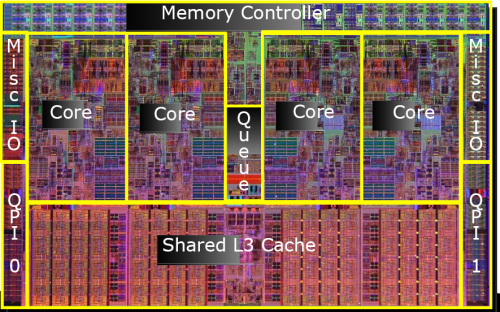
\includegraphics[width=0.45\textwidth]{cpu_diagram.png}
\caption{Quad-core Intel Core i7 CPU Architecture Diagram}
\label{fig:cpu_diagram}
\end{figure}

% [Use of GPUs – GPU Architecture]

Graphical Processing Units (GPU) are a newer technology than CPUs and serve a dedicated purpose of taking instructions from the CPU and performing multiple, hardware-based mathematical operations for translating three-dimensional shapes and coordinates into two-dimensional projections for rendering to a display, and runs multiple small programs called ``shaders” to handle colour and lighting. Due to the sheer amount of mathematical calculations that need to be performed to display something onto a display, GPUs are architected differently to a CPU. Modern graphics cards, such as NVIDIA’s Turing architecture, pictured in Figure \ref{fig:gpu_diagram}, are composed of multiple stream processors, each divided into hundreds of small cores which perform a single integer or floating-point operation. This stream processing approach allows for vast parallel computation over a large dataset in a paradigm called ``single instruction multiple data” (SIMD).

This parallelism was previously reserved for image and video processing but a few years ago NVIDIA released their CUDA API\cite{cuda_talk}\cite{CUDA} which allows developers to leverage the stream processing nature of the GPU for general-purpose computation. Scientific workloads from biomedical imaging\cite{luebke2008cuda} to deep learning\cite{tang2013deep} are now done on the GPU, and modern supercomputers, such as Summit, are built with large numbers of GPUs to accelerate workloads and perform previously-impossible simulations and workloads.

% \footnote{\url{https://devblogs.nvidia.com/nvidia-turing-architecture-in-depth/}}
\begin{figure}
\centering
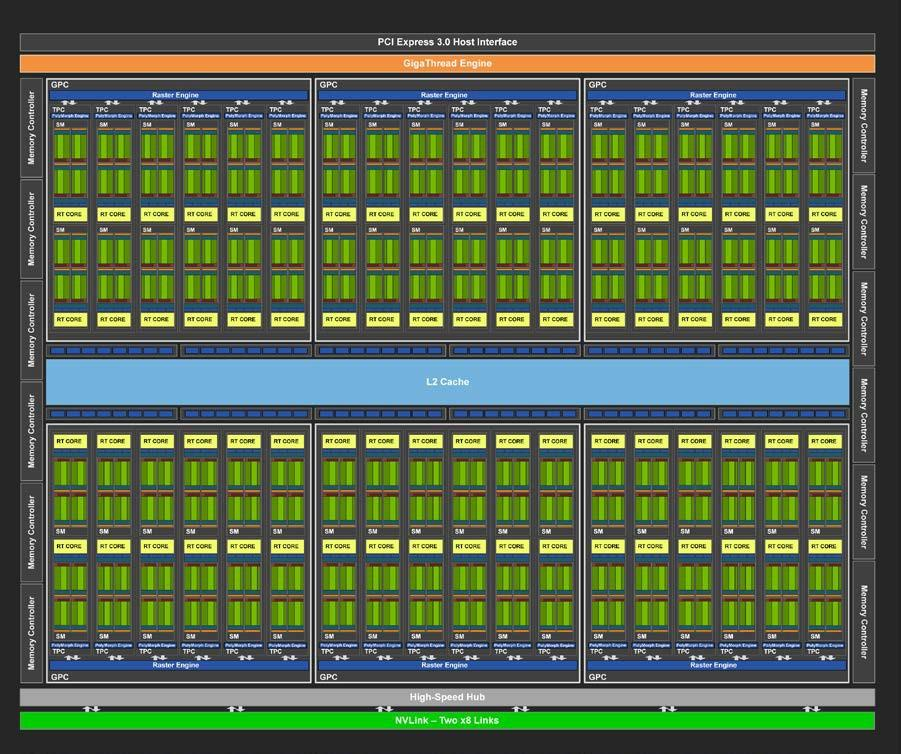
\includegraphics[width=0.45\textwidth]{gpu_diagram.jpg}
\caption{NVIDIA Turing GPU Streaming Multiprocessor Architecture Diagram}
\label{fig:gpu_diagram}
\end{figure}

% Miniapps
Mini-applications (``miniapp”) are a new area within the field of High Performance Computing (HPC). These applications are small, self-contained proxies for real applications (typically relating to simulation of physical phenomena) to quickly and concisely explore a parameter space, leading to focused and interesting performance results to investigate potential scaling and run-time issues or trade-offs\cite{miniapps}. Miniapps capture the behaviour and essence of their parent applications primarily because of two characteristics of many applications running on distributed systems: the performance of an application will mainly be constituted by the performance of a small subset of the code, and many of the physical models that constitute the rest of the application are mathematically distinct and generally have similar performance characteristics\cite{miniapps}.

\subsection{Aims}

The SN (Discrete Ordinates) Application Proxy (SNAP) is a miniapp that acts as a proxy for discrete ordinates particle transport. It is modelled off another production simulation program developed by the Los Alamos National Laboratory called PARTISN, which solves the linear Boltzmann transport equation (TE)\footnote{Boltzmann Equation: \url{ https://en.wikipedia.org/wiki/Boltzmann_equation}}, simulating neutron criticality and time-independent neutron leakage problems\cite{partisn} in a multi-dimensional phase space. SNAP is a proxy to PARTISN because it provides a concise solution to a discretised, approximated version (though with no real-world relevance) of the same problem PARTISN solves, providing the same data layout, the same number of operations, and loads elements into arrays in approximately the same order.

The SNAP algorithm works by defining the phase space as seven dimensions: three in space (x, y, z), two in angle (octants, angles), one in energy (groups, or energy-based bins of particles), and one of time (time step). SNAP sweeps across the spatial mesh, starting in each of the octants proceeding towards the antipodal octant, performing a time-dependent calculation in each cell using information form the previous time-step and surrounding cells. This motion forms a wave-front motion that sweeps across the three-dimensional space from corner to corner, with work being divided along each diagonal for parallel execution

The primary aim of this project is to take the SNAP project and convert the parallelisation from an OpenMP-based multi-core CPU implementation, to a CUDA-based GPU implementation and investigate the (potential) performance improvements and scalability of such an enterprise.

\subsection{Problem Statement}

This research proposal defines three key problems that the final output of the project intends to solve. Taken together, these will provide a holistic overview as to the validity and efficacy of this approach of converting CPU-bound parallelised algorithms to utilise the GPU instead (where appropriate). With the SNAP algorithm and open-source repository (specifically the C-based port of the code) in mind, the three key problems this project seeks to solve are:

\begin{itemize}

\item To instrument, profile, and analyse the current implementation of the code in order to identify areas of the code in which it would be applicable and beneficial to convert to CUDA-based parallelisation.

\item Using the identified areas found in problem 1, to fork the current SNAP GitHub repository\footnote{\url{https://github.com/lanl/SNAP}} and convert the candidate components and routines from OpenMP to utilise the CUDA libraries instead.

\item Following the reimplementation of the algorithm to CUDA technology, the last step is to analyse and evaluate the efficiency and efficacy of the new solution in comparison to the previous CPU-based approach. Ideally, a theoretical maximum efficiency of the approach will also be calculated mathematically, and the actual implementation compared against this as another measure of success.

\end{itemize}

%%%%%%%%%%%%%%%%%%%%%%%%%%%%%%%%%%%%%%%%%%

\section{Related Work}

A seminal work in the field of miniapps was written by Heroux et al\cite{miniapps}, defining the paradigm. Their Mantevo miniapp suite has show successful development of miniapps, such as MiniFE for finite element analysis and MiniMD for molecular dynamics simulations, to demonstrate their versatility and applicability. Others have demonstrated such success in other areas, such as Mallinson et al with ``CloverLeaf”\cite{mallinson2013cloverleaf}, and Los Alamos National Lab (\url{https://www.lanl.gov/projects/codesign/proxy-apps/lanl/index.php}). Miniapps have been shown to produce similar performance characteristics to their fully-ledged counterparts\cite{miniapps}, adding to the efficacy of the paradigm.

General-purpose simulations on GPUs have been studied for a long time, with GPUs being a core part of modern computing clusters\cite{debardeleben2013gpu}. Strong-scaling across multiple GPUs\cite{glaser2015strong} is the ideal approach. Consideration is taken also for conversion of existing codebases\cite{zhou2011gpu} and new, bespoke solutions designed with GPU architecture utilisation in mind\cite{glaser2015strong}. Bespoke solutions offer superior code architecture and speed, meaning calculation of theoretical maximum performance increase for a pre-existing code base will have to take this into account.

Writing GPU targeted miniapps in a developing area of work. Baker et al\cite{baker2012high} discuss implementation details of converting the KBA sweep algorithm of the Denovo code system to run on NVIDIA’s Titan GPU. Mallison et al\cite{mallinson2013cloverleaf} demonstrate too with CloverLeaf the performance advantages GPU-based architecture targeting can have over purely CPU-based versions. It is important to note that these performance increases might not necessarily be completely reflected in SNAP’s algorithm due to other considerations, such as the scaling characteristics of the algorithm\cite{shoukourian2014predicting} and communication technologies as highlighted by Glaser et al\cite{glaser2015strong}.

Performance of miniapps with respective to CPU and GPU-based parallelisation frameworks have been explored previously and show promising results which add credence to the motivation of this project. Notably Martineau et al\cite{martineau2017productivity} reaching the conclusion that compiling miniapps to CUDA resulted in greater efficiencies compared to other targets, though care is needed to consider the implementation (especially with respect to data accesses) to avoid the compiler introducing performance penalties.

Development of the solution must still mimic the behaviour of the original application however, so care must be taken to preserve this. Heroux et al\cite{miniapps} and Messer et al\cite{messer2015developing} outline the fundamental principles that a miniapp must adhere to and the considerations of forming a miniapp from the base application – all of which would help form testing criteria for this project and future projects to help preserve results and intrinsic behaviour.

%%%%%%%%%%%%%%%%%%%%%%%%%%%%%%%%%%%%%%%%%%

\section{Project Review}


\subsection{Current Progress}

\subsection{Reflection of Current Efforts}
\begin{itemize}
\item Presentation went well
\item Highlighted problem with gantt chart/timetable - wasn't realistic, exams got in the way
\end{itemize}

%%%%%%%%%%%%%%%%%%%%%%%%%%%%%%%%%%%%%%%%%%

\section{Going Forward}

%%%%%%%%%%%%%%%%%%%%%%%%%%%%%%%%%%%%%%%%%%



% Research approach/methodology, etc...
% \section{Research Processes}

% The research methodologies utilised in this project can be categorised into two stages.

% The first stage is for the research undertaken as part of this proposal to assess the academic field relating to high-performance computing and GPU-based parallelisation. The Library at University of Warwick offers a collection of databases of scholarly content (articles, journals, data etc.) for students to search through. These databases are trusted, informative sources of research – from IEEE to ACM – that allows for search by keywords and phrases. Using a handful of seminal papers that are central to the HPC and miniapp fields, searches were done relating to these terms, and citations from previous papers followed, to accumulate varied and relevant research to ascertain the current state-of-the-art, theories, proof-of-concepts, and existing work. This is in aid of cementing and consolidating knowledge of the field, identifying key analytical techniques and metrics to suitably measure and evaluate the final output of the project (especially against existing systems) and to identify gaps in the literature that this project ultimately aims to contribute to.

% The other stage is for the methodology with which the project will be undertaken. Principally with regards to how the initial analyses and performance profiling of the SNAP project will be done and how the modified project will be tested and assessed.

% In terms of the analysis and profiling of the code in its current state, a swathe of programs and modifications will be performed in order to fully understand the time each section of the code takes to run and how the OpenMP library parallelises the code (this last stage is in conjunction with a manual inspection of the code as well as flow-charting key aspects of the algorithm). From this, a well-defined theoretical understanding will be ascertained that would allow us to derive a more granular model of parallelisation to use on the critical areas of the codebase to allow for our GPU-based model to be most effective.

% Testing the final solution will be performed in comparison to the current codebase ideally on different host machines. Running both applications, with the same input data and controlling as many external variables as possible (such as keeping the amount of background processes consistent, performing multiple runs to calculate an average etc.), on a consumer-focused target machine with a multicore CPU and dedicated GPU will provide an initial result to show if the modifications produce the desired speed increase. From this, it is hoped to conduct further research into the efficacy of the solution by running the program on University of Warwick’s Tinis or Orac computing clusters. Execution on a cluster will demonstrate, if any, the scalability of the solution, and if there is any difference between running on highly multicore CPUs (several Intel Xeon processors) and running on several compute-specific GPU cards (NVIDIA P100 or Tesla K68 GPUs, for example).

% Our research will conclude by compiling, contrasting, and comparing the performance characteristics of both applications to gauge the superior software architecture for SNAP, and from this, hope to learn about the advantages and disadvantages of GPU-based miniapps.


% Timeline, constraints, risk, etc...
% \section{Project Management}

% \subsection{Management and Accountability}

% For the project to progress, it is important that consistent work is made and is made in the right direction. The code for the project will be uploaded to a public-facing GitHub repository to keep track of the progress of the project, in addition to being able to properly source control the software to allow for experimental branches, backing up of code, and to manage future releases.

% Communication with the supervisor for this project will be done on a weekly basis via email, Skype, or in-person meetings to discuss the progress of the previous week, demonstrate current findings or developments, and to deliberate next steps.

% The final write-up for this project will be done in a pipelined fashion, wherein different sections and aspects of the dissertation are written whilst others are submitted to the supervisor for consideration and approval for accuracy and readability.

% \subsection{Timeline}

% An estimated timeline of the project follows overleaf.

%\newgeometry{vmargin=1cm, hmargin=1cm}
%\begin{landscape}
%\thispagestyle{empty}\centering
%
%\ganttset{calendar week text=\small{\startday}}
%\begin{ganttchart}[
%    hgrid,x unit=0.1cm,
%    hgrid style/.style={draw=black!5, line width=.75pt},
%    vgrid={draw=none,draw=none},
%    bar label node/.style={text width=3cm,align=right,font=\scriptsize\RaggedLeft,anchor=east},
%    group label node/.style={text width=3cm,align=right,font=\bf\scriptsize\RaggedLeft,anchor=east},
%    time slot format=little-endian]{18-02-2019}{30-09-2019}
%\gantttitlecalendar{month=shortname, week=4} \\
%\ganttgroup{Total Duration}{18-02-19}{30-09-19}\\
%% Investigation and Design
%\ganttgroup{Investigation and Design}{21-02-19}{08-04-19}\\
%\ganttbar{Initial Investigation}{21-02-19}{05-03-19}\\
%\ganttbar{In-depth Profiling and Analysis}{24-02-19}{03-04-19}\\
%\ganttbar{Researching Libraries and Techniques}{28-03-19}{08-04-19}\\
%% Design and implementation
%\ganttgroup{Design and Implementation}{25-03-19}{30-06-19}\\
%\ganttbar{Initial Design}{25-03-19}{30-04-19}\\
%\ganttbar{Programming}{22-04-19}{30-06-19}\\
%% Testing
%\ganttgroup{Testing}{15-05-19}{14-07-19}\\
%\ganttbar{Local Profiling and Benchmarking}{15-05-19}{14-06-19}\\
%\ganttbar{Cluster Profiling and Benchmarking}{14-06-19}{14-07-19}\\
%% Dissertation
%\ganttgroup{Dissertation}{17-06-19}{30-09-19}\\
%\ganttbar{Writing}{17-06-19}{17-09-19}\\
%\ganttbar{Proof Reading and Editing}{01-09-19}{30-09-19}
%\end{ganttchart}
%\end{landscape}
%\newgeometry{vmargin=2.25cm, hmargin=2.25cm}

% Overview of progress, etc...
% \section{Progress}

% Currently, the field of high-performance computing with respect to GPU-based parallelisation workloads has been initially researched (see the ``Related Work” section above). From this, several considerations regarding the profiling and benchmarking process of analysing the SNAP project to identify easily GPU-parallelisable workloads has been developed and will guide the design stage of the project and the likely implementation that will result.

% An investigation into the pipeline and API of NVIDIA’s CUDA technologies has been started also. It is important to fully understand the central tenants and paradigms of a technology before any implementation that aims to use it can get underway. This stage will progress smoothly because of NVIDIA’s dominance in the market place, the age and maturity of the technology, and its prevalence in HPC applications.

% Finally, a clone of the SNAP GitHub repository has been downloaded and study of the provided documentation and algorithm (from the C-based port of the code, which is what this project will focus on) has begun. The next stage in this process is to choose the appropriate running environment for the application, to start and successfully execute the application with a sample workload, and to begin instrumentation and profiling of the code.

% Summary, future work, etc...
% \section{Conclusion}
% Whilst the aim of this research proposal is to ascertain the potential performance increases of converting the SNAP miniapp to run on a GPU-based architecture, it also highlights the opportunity to formalise and contribute towards different aspects of the miniapp field that have been explored but not yet fully developed.

% Introduction of new or use of existing software profiling and diagnostic techniques will be used to identify areas of the codebase that have the potential for increased parallelism – potentially the basis for an automated system to translate serial or partially-parallel code to fully parallel for the most applicable available architectures. Development and testing of the implementation will follow, which will hopefully lead to a successful, open-source reimplementation of the SNAP algorithm, and ideally produce recommendations for parallelising certain components or algorithms based on data structures, algorithm design, or strong or weak scaling characteristics of certain parts of a code base.

% The research proposal finally outlines the direction of the project and the current progress made.

% \nocite{*}

\bibliographystyle{unsrt}
\bibliography{interim_report}

\end{document}